
\chapter{Projections of the main fit to data}
\label{app:main_fit}

This appendix includes projections of the main fit to data described in Section~\ref{sub:main_cpfit_results}, for each of the 160 subcategories in the fit. The projections for LL candidates where \DtoKspp are shown in Figs.~\ref{fig:all_proj_LL_1}~and~\ref{fig:all_proj_LL_2}; the equivalent projections for DD candidates are shown in Figs.~\ref{fig:all_proj_DD_1}~and~\ref{fig:all_proj_DD_2}; finally the projections for candidates where \DtoKskk are shown in Figs.~\ref{fig:all_proj_LL_kskk}~and~\ref{fig:all_proj_DD_kskk}. 


\begin{figure}[tp]
    \centering
    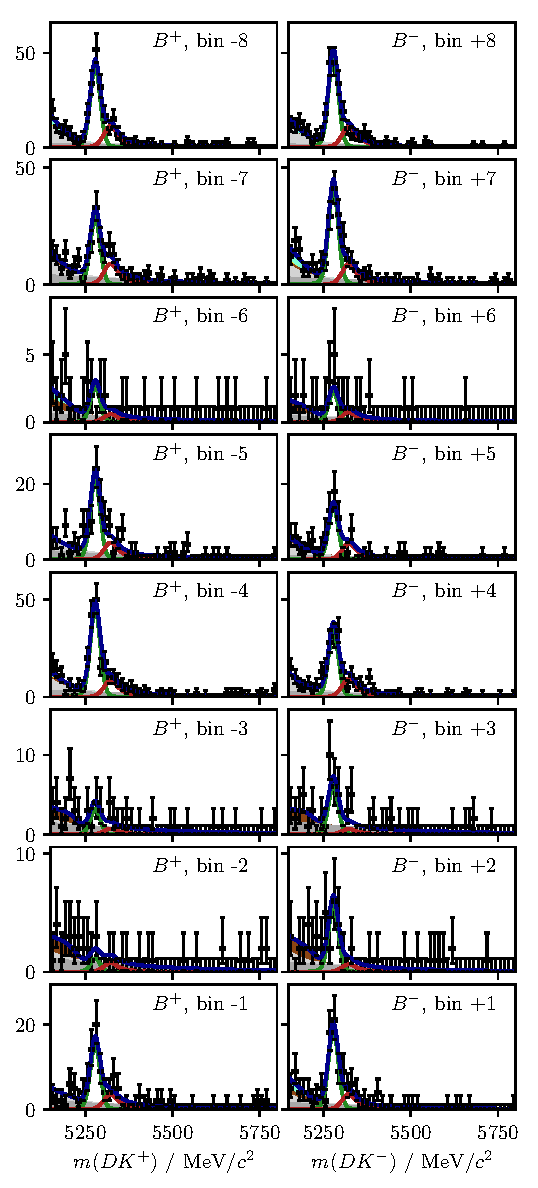
\includegraphics[height=6in]{figures/analysis/bin_by_bin/pretty_fit_bins_dk_LL_1.pdf}
    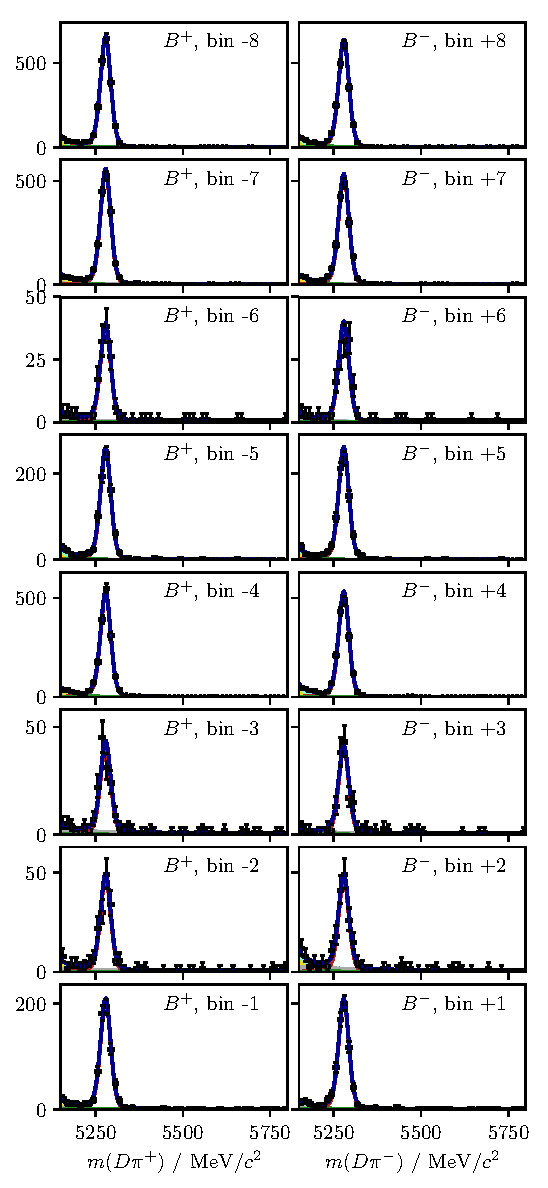
\includegraphics[height=6in]{figures/analysis/bin_by_bin/pretty_fit_bins_dpi_LL_1.pdf}
    \caption{Projections of the main fit to data described in Section~\ref{sec:measurement_of_the_cp_violation_observables}. The two columns on the left show \BtoDK candidates, split by charge, while the two columns on the right show \BtoDpi candidates. These projections are for the \DtoKspp mode where the \KS meson is in the LL category.}
    \label{fig:all_proj_LL_1}
\end{figure}

\begin{figure}[tp]
    \centering
    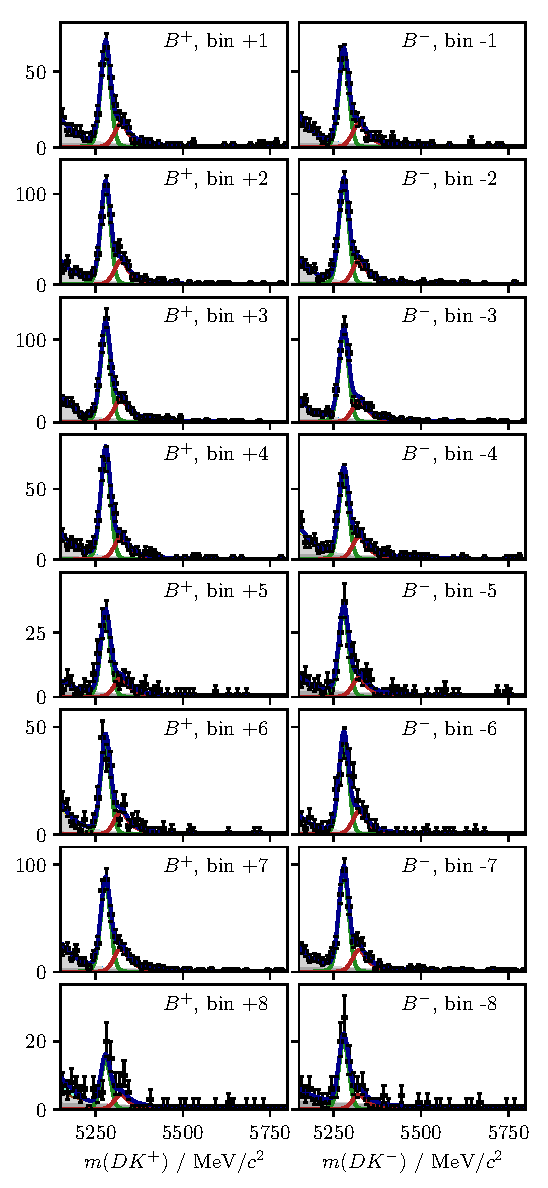
\includegraphics[height=6in]{figures/analysis/bin_by_bin/pretty_fit_bins_dk_LL_2.pdf}
    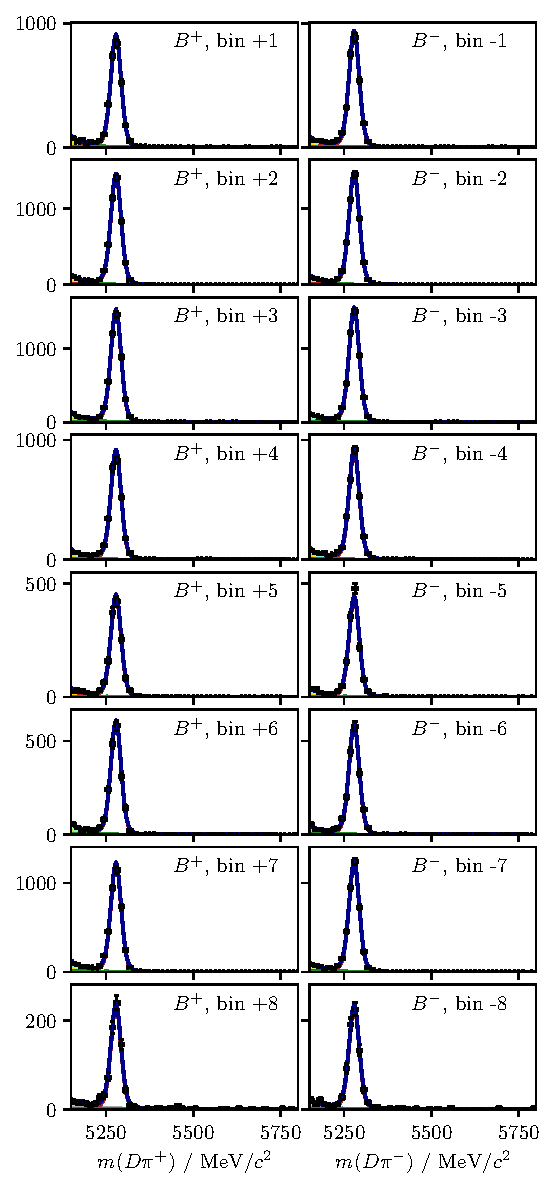
\includegraphics[height=6in]{figures/analysis/bin_by_bin/pretty_fit_bins_dpi_LL_2.pdf}
    \caption{Projections of the main fit to data described in Section~\ref{sec:measurement_of_the_cp_violation_observables}. The two columns on the left show \BtoDK candidates, split by charge, while the two columns on the right show \BtoDpi candidates. These projections are for the \DtoKspp mode where the \KS meson is in the LL category.}
    \label{fig:all_proj_LL_2}
\end{figure}

\begin{figure}[tp]
    \centering
    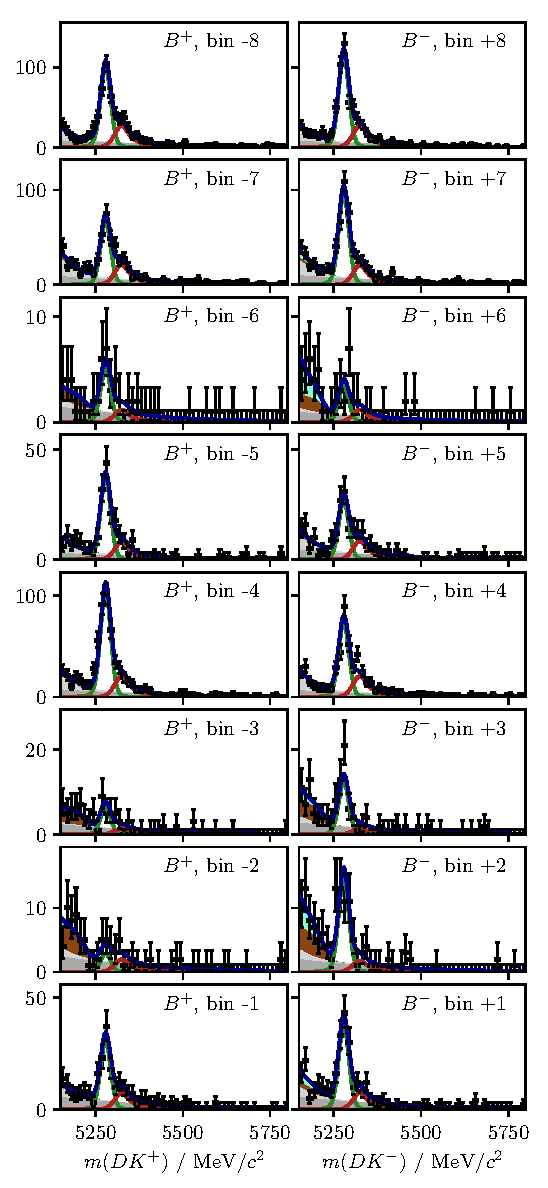
\includegraphics[height=6in]{figures/analysis/bin_by_bin/pretty_fit_bins_dk_DD_1.pdf}
    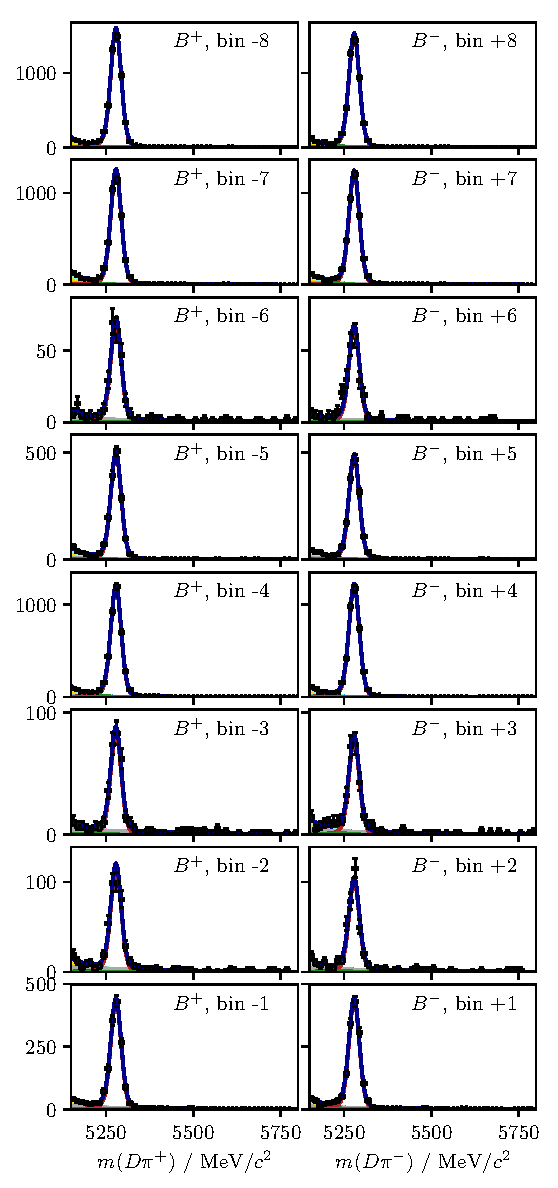
\includegraphics[height=6in]{figures/analysis/bin_by_bin/pretty_fit_bins_dpi_DD_1.pdf}
    \caption{Projections of the main fit to data described in Section~\ref{sec:measurement_of_the_cp_violation_observables}. The two columns on the left show \BtoDK candidates, split by charge, while the two columns on the right show \BtoDpi candidates. These projections are for the \DtoKspp mode where the \KS meson is in the DD category.}
    \label{fig:all_proj_DD_1}
\end{figure}

\begin{figure}[tp]
    \centering
    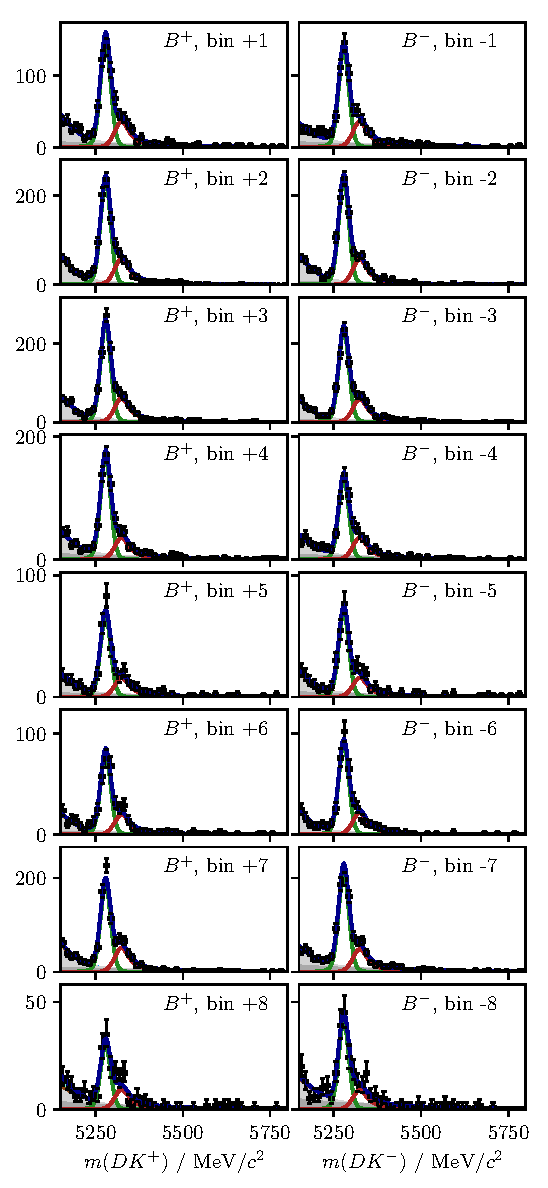
\includegraphics[height=6in]{figures/analysis/bin_by_bin/pretty_fit_bins_dk_DD_2.pdf}
    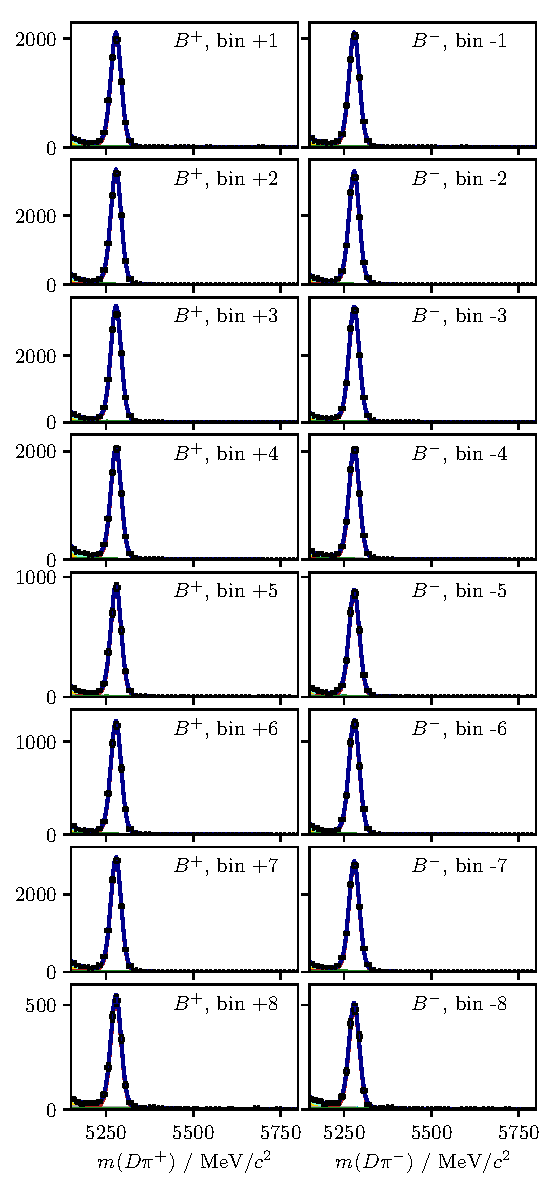
\includegraphics[height=6in]{figures/analysis/bin_by_bin/pretty_fit_bins_dpi_DD_2.pdf}
    \caption{Projections of the main fit to data described in Section~\ref{sec:measurement_of_the_cp_violation_observables}. The two columns on the left show \BtoDK candidates, split by charge, while the two columns on the right show \BtoDpi candidates. These projections are for the \DtoKspp mode where the \KS meson is in the DD category.}
    \label{fig:all_proj_DD_2}
\end{figure}

\begin{figure}[tp]
    \centering
    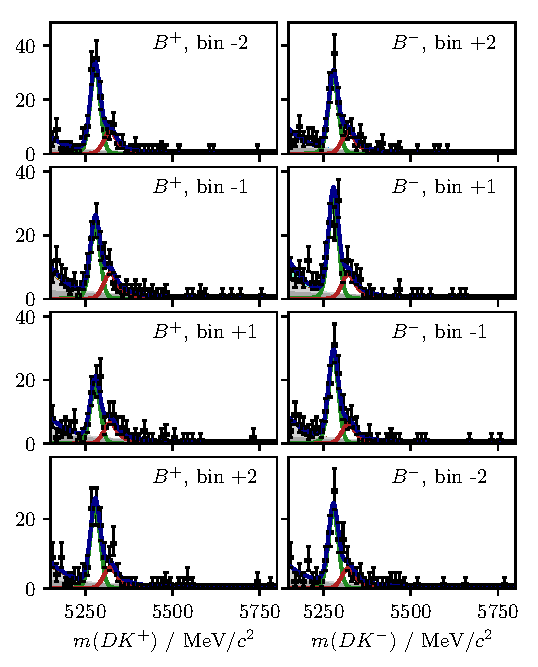
\includegraphics[height=3.5in]{figures/analysis/bin_by_bin/pretty_fit_bins_dk_LL_1_d2kskk.pdf}
    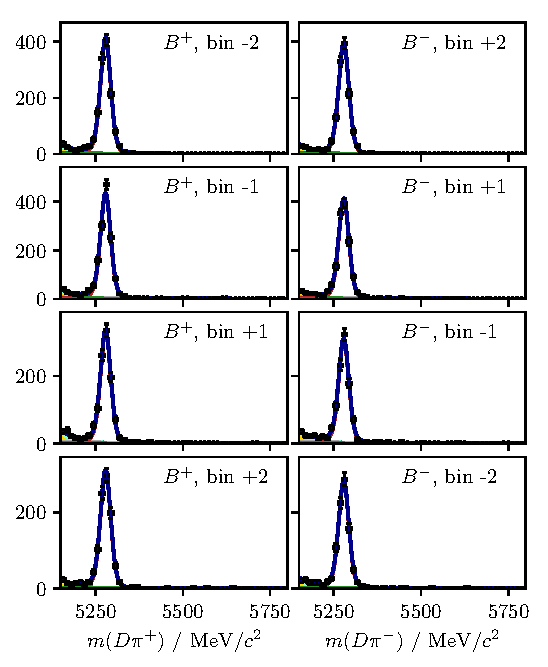
\includegraphics[height=3.5in]{figures/analysis/bin_by_bin/pretty_fit_bins_dpi_LL_1_d2kskk.pdf}
    \caption{Projections of the main fit to data described in Section~\ref{sec:measurement_of_the_cp_violation_observables}. The two columns on the left show \BtoDK candidates, split by charge, while the two columns on the right show \BtoDpi candidates. These projections are for the \DtoKskk mode where the \KS meson is in the LL category.}
    \label{fig:all_proj_LL_kskk}
\end{figure}

\begin{figure}[tp]
    \centering
    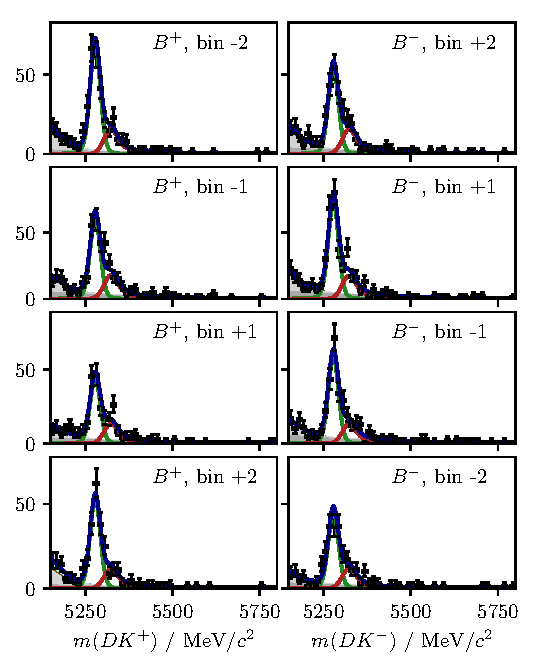
\includegraphics[height=3.5in]{figures/analysis/bin_by_bin/pretty_fit_bins_dk_DD_1_d2kskk.pdf}
    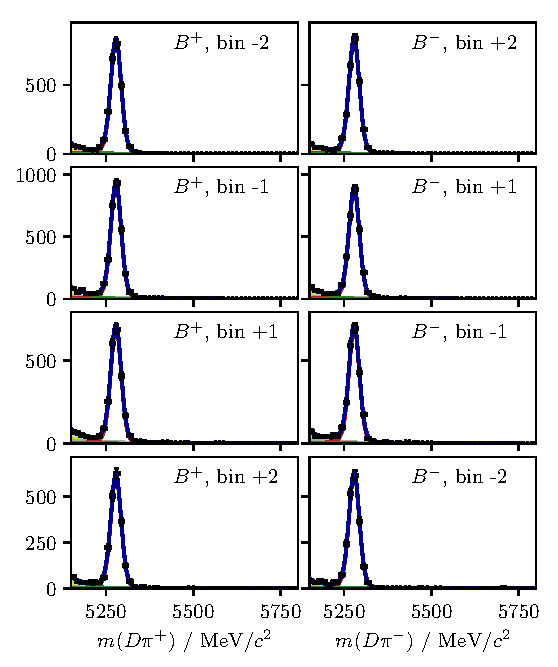
\includegraphics[height=3.5in]{figures/analysis/bin_by_bin/pretty_fit_bins_dpi_DD_1_d2kskk.pdf}
    \caption{Projections of the main fit to data described in Section~\ref{sec:measurement_of_the_cp_violation_observables}. The two columns on the left show \BtoDK candidates, split by charge, while the two columns on the right show \BtoDpi candidates. These projections are for the \DtoKskk mode where the \KS meson is in the DD category.}
    \label{fig:all_proj_DD_kskk}
\end{figure}